
\subsection{Particle Beam Requirements}
The requested beam parameters are driven by the requirement that the results from the CERN test beam should be directly applicable to the future large underground single-phase LAr detector with minimal extrapolation. The CERN test beam data will be used to evaluate the detector performance, to understand the various physics systematic effects, and to provide ``neutrino-like'' data for event reconstruction studies. The chosen beam parameters span a broad range of particle spectrum that are expected in the future neutrino experiment. The particle beam composition should consist of electrons, muons, and hadron beams that are charge-selected. The particle momentum of interest ranges from 0.2 GeV/c to 10 GeV/c. The maximum electron drift time in the TPC is about 3 ms. To minimize pile-up in the TPC, the desired beam rate should be around 200 Hz with the maximum rate below 300 Hz. The single-phase TPC consists of two drift volumes. It is desirable to aim the particle beam so that hadronic showers are mostly contained in the same drift volume.  However, we also plan to take some data with hadronic shower crossing the midplane of the TPC from one drift volume to another.  The two beam entry angles and positions with respect to the LAr cryostat are illustrated is Figure [XYZ.] The summary of the beam requirements are shown in Table~\ref{table:beamspecs}.

\begin{table}[h]
\centering
\caption{Particle beam requirements.}
\label{table:beamspecs}
\begin{tabular}{|c|c|c|}
\hline
\textbf{Parameter } & \textbf{Requirements} & \textbf{Notes}  \\ \hline
  Particle Types        & $e^\pm,\mu^\pm,\pi^\pm$          &                   \\ \hline
  Momentum Range   & 0.2 - 10 GeV/$c$  &   \\ \hline
  Momentum Spread   & $\Delta p/p  < $5 \%  &   \\ \hline
  Transverse Beam Size   & RMS(x,y) $<$ 2.5 cm &  At the entrance face of the \\ 
                                              &                                        & LAr cryostat \\ \hline
  Beam Divergence &   &   \\ \hline
  Beam Angle &  $\approx20^{\circ}$  &   \\ \hline
  Beam Dip Angle &  -6$^\circ$ (nominal); $\pm5^\circ$ range &   \\ \hline
  Beam Entrance Position &   &   \\ \hline
  Rates & 200 Hz (average); 300 Hz (maximum)  &   \\ \hline
\end{tabular}
\end{table}

\subsection{EHN1 H4ext Beamline}
The H4ext is an extension of the existing H4 beamline in Experimental Hall North 1 (EHN1).  To produce particles in the momentum range of interest, 60 - 80 GeV/c pion beam from the T2 target is used to generate tertiary beams. The tertiary particles are momentum and charge-selected and transported down H4ext beamline to the experimental area. A preliminary layout of the H4ext beamline is shown in Figure~\ref{fig:H4extPrelim}.

\begin{figure}[h]
  \centering
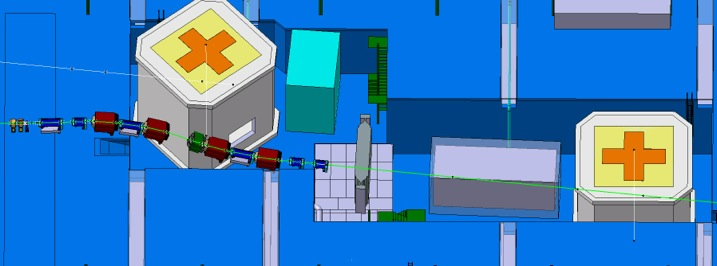
\includegraphics[scale=0.7]{figures/EHN1Ext_Prelim.jpg}
  \caption{Preliminary layout of the H4ext beamline  }
  \label{fig:H4extPrelim}
\end{figure}

\subsubsection{Beam Optics}
[Waiting for inputs from Ilias]

\subsubsection{Expected Rates and Purity}
[Waiting for inputs from Ilias]

\subsection{Beam Instrumentation}
\subsubsection{Beam Position Detector}
\subsubsection{Time-of-Flight Detector}
\subsubsection{Threshold Cherenkov Counter}

\subsection{Muon Beam Halo Counters}
The halo counter is a set of plastic scintillator paddles surrounding the beamline. The main purpose is to tag particles (primarily muons from the upstream production target) that are outside of the beam axis, but may potentially enter the TPC volume. The counter information is used to either veto or simply flag these class of events.

\subsection{Beam Window on LAr Cryostat}
This section could be absorbed into the cryostat chapter.
